\chapter{Introduction}

\section{Introduction to Research Statement}
A mechanism is defined to be a collection of rigid bodies connected by joints such as hinges or sliders in order to generate articulated motions. Kinematic synthesis of mechanism deals with computing type and the dimension of mechanisms that are useful for a particular task\footnote{a general term describing prescribed path for path generation problem, prescribed motion for motion generation problem and prescribed function for function generation problem}(\ac{x_task}).
The past forty years of research in kinematic synthesis of mechanisms has witnessed an unprecedented volume of work in formulating and solving planar linkage synthesis problems.
However, finding practical and useful mechanisms for the synthesis problems has proven to be a difficult feat.

Mechanism synthesis is a critical part of the conceptual design phase, which requires synthesis methods to be prolific in terms of concept generation to 1) realize the potential of attainable design possibilities, and 2) have the agility to adapt a design to evolving requirements.
To achieve the above goal, the proposed research brings together machine learning and theoretical kinematics to create a data-driven computational framework for kinematic synthesis of mechanisms.
This work comprises of algorithmic developments presented in Chapter~\ref{ExtendedBurmester} that solve some of the outstanding challenges faced by the previously developed state of the art methods for kinematic synthesis of mechanisms.
In the next phase of the work, a data-driven approach is presented which couples the synthesis algorithms with novel machine learning models that enhance the prolificacy and transparency of the crucial conceptual design phase.

This is achieved by 1) inception of an End to End synthesis pipeline that accepts deliberately imprecise or inherently uncertain input from users and provides them with a large variety of acceptable solution concepts, and 2) an approach using state-of-the-art deep generative models that learn joint probability distribution of various linkage parameters and their interdependence to perform tasks such as input conditioning, imputation, and variational synthesis.
In doing so, we leverage the emerging machine learning techniques to learn meaningful representations and combine them with simultaneous type and dimensional methods of kinematic synthesis to enhance users' computational creativity.
This also enables us to answer the following questions: 
1) what are the infeasible aspects of the input and how to modify them to make a more conducive input,
2) given a path or a motion task, how likely it is that a particular type of mechanism can perform the task, 3) for a given task, what is the distribution of linkage parameters with similar coupler motions (or, paths).

\section{Motivation}
Depending upon the nature of the task, synthesis problems have been divided into mainly three categories: 1) Function Generation, 2) Path Generation, and 3) Motion Generation.
The Function Generation task demands a prescribed relationship between the rotation of input and output links of the mechanism.
In the Path Generation task, the aim is to move an object through space along a prescribed path, whereas in Motion Generation a rigid body needs to be guided along a prescribed motion.
Hereinafter, Motion is termed as a continuous sequence of poses, where a \ac{pose} is a combination of position and orientation.

A general synthesis procedure can be represented as,
\begin{equation}
     \textbf{Solver}(X_{\text{task}}) =  {\{L^{i}_{\text{para}}\}}_{i=1}^{i=n}.
\end{equation}
Here, a synthesis solver $\textbf{Solver}$ takes the task \ac{x_task} as the input and produces n solutions. $L^{i}_{\text{para}}$ is the set of linkage parameters for the $i^{th}$ solution. 
\ac{X}\footnote{$X$ is a general term representing target property of linkage for which the kinematic synthesis is conducted. In case of motion (or path) generation problem, $X$ is coupler motion (or path)} is the targeted linkage property prescribed by \ac{x_task}.
Methods for mechanism synthesis start with taking input \ac{x_task} in the form of a sequence of path-points, poses, or functional input-output relationship from the user. A large majority of Motion and Path Generation methods take the precision point approach, which optimally minimizes the least squared fitting error between \ac{x_task} and \ac{X}.
This approach is highly susceptible to input precision points/poses and in most cases results in solutions with circuit or branch defects~\cite{chasemirth}. The root cause of sensitivity is in the underlying nature of the interpolation problem.

To illustrate this chaotic nature, let us consider the following example.
Six poses are sampled from a four-bar linkage as shown in Fig.~\ref{fig_chaotic_motiongen}.
\begin{figure*}[tbh]
\centering
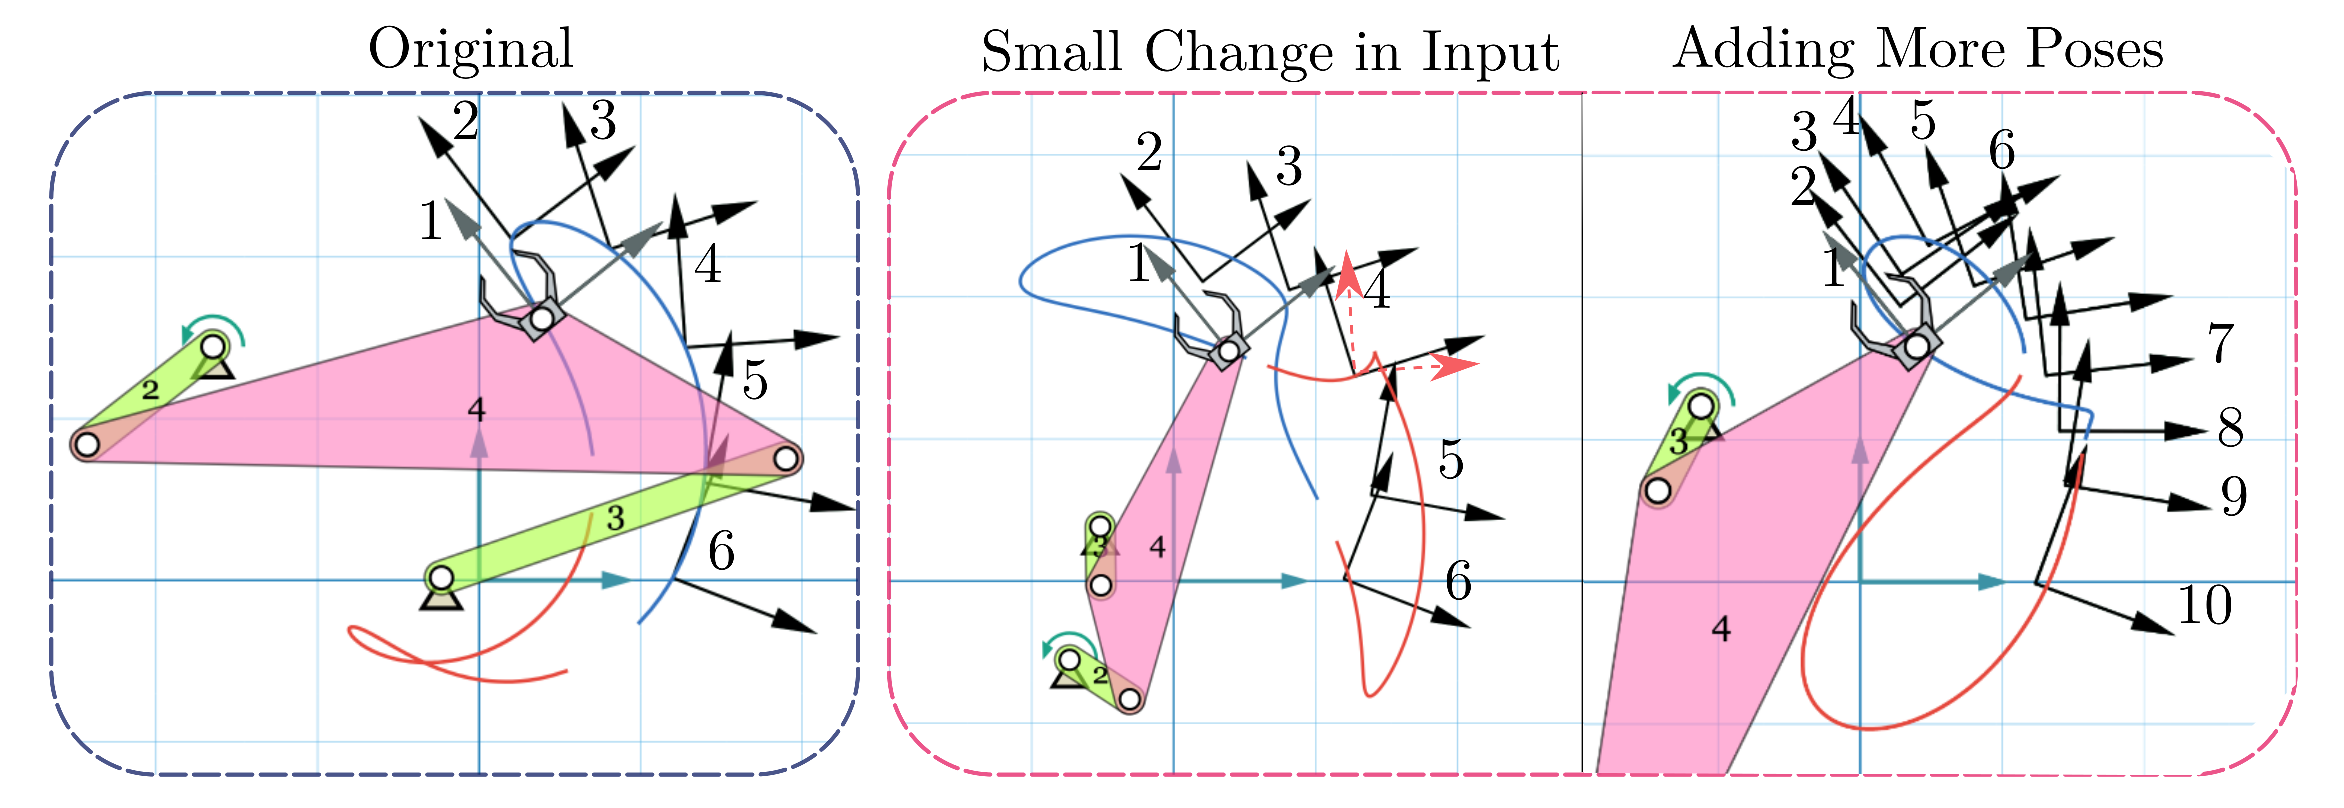
\includegraphics[width=0.75\textwidth]{jmd-19/figure/motiongen-chaos.eps}
  \caption{Slightly different inputs result in entirely different mechanisms. The input on the left generates a defect-free four-bar linkage. The input in the middle is formed by perturbing the orientation of the fourth pose by 15 degrees. The dashed frame in the middle input represents the original unaltered pose. Increasing the number of poses does not help either as shown by the mechanism generated on the right.}
\label{fig_chaotic_motiongen}
\end{figure*}
As the poses are already known to lie on the coupler motion, our motion generator algorithm\cite{shrinathpurwar2017} explained in chapter~\ref{ExtendedBurmester} obtains the original four-bar as expected.
However, even a small change in the orientation of a pose results in an entirely different linkage suffering from branch defect, therefore making it unsuitable to perform the function.
Moreover, increasing the number of positions by means of a B-spline interpolation through original poses does not help as shown in the last of Fig.~\ref{fig_chaotic_motiongen}.
It is important to note that the algorithm~\cite{shrinathpurwar2017} used for synthesis in the example is a representative of the approaches based on the precision point approach.
In the real world, when a user inputs a sequence and receives a result not suitable for the application, no informed decisions can be made to rectify the situation.
To add more uncertainty, the task is often an approximation of the designer's intended motion.
To accommodate this uncertainty, a common approach is to do random perturbations within the tolerance of target path or motion in the hope of getting a good solution.
The probability of a random perturbation to find a valid input reduces exponentially with the number of precision positions as well as the tolerance range.

To perform informed and meaningful modification to \ac{x_task}, it is necessary to possess knowledge about the properties of \ac{X}. Let us define this knowledge as a \emph{prior probability distribution}. In Bayesian statistical inference, a prior probability distribution, often simply called the \ac{prior}, of an uncertain quantity is the probability distribution that would express one's beliefs about this quantity before some evidence is taken into account.

While the sensitivity to the input has been a problem in finding good solutions, it turns out that we can exploit the susceptibility of synthesis algorithms by providing them with a variety of preconditioned inputs so as to find a \emph{diverse} range of defect-free solutions. By providing tools that can provide the designer with higher level control on input specification, we can help them be more creative as well.


\section{Overview}

\begin{figure}
\centering
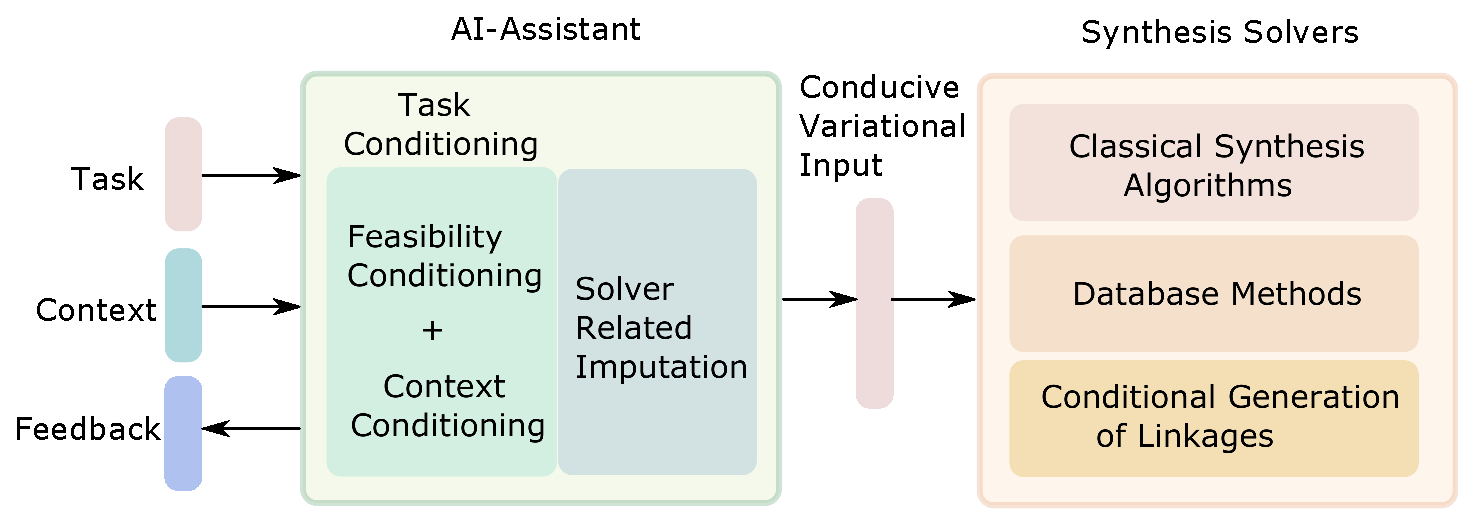
\includegraphics[width=0.9\textwidth]{figure/overview.eps}
  \caption{The framework accepts the task and the context. AI-assistant performs task conditioning to compute a distribution of conducive inputs. Task conditioning also provides feedback on the quality of inputs. Samples from this distribution are fed to suitable synthesis algorithms to obtain a variety of concept solutions.}
\label{fig_overview}
\end{figure}

The key contribution of the framework is in the development of an AI assistant which acts as an intermediary between designer and computational solvers. An overall view of the approach is depicted in Fig.~\ref{fig_overview}. As it can be seen in Fig.~\ref{fig_overview}, the framework accepts \ac{x_task} and the context for the synthesis problem. The context provides a secondary prescription in the form of fitness function (\ac{context_function}) that evaluates the fitness of a solution. For example, it can be used to prescribe the desired region for fixed pivots to lie on. The framework allows for any such differentiable fitness function of $X$ that is known or can be learned from data. 


Next, \ac{x_task} is subjected to task conditioning. This is done as follows. The framework captures the salient features \ac{z} in the task by the means of variational inference and computes a distribution of conditioned inputs for computational solvers. The task is conditioned so that the likelihood of getting a desirable solution from the solver is maximized. The desirable solution is defined as the linkage which is free of defects and satisfies the conditions implied by the context. Here, we define feasibility conditioning as modifying the task to make it more conducive for obtaining defect-free solutions by synthesis. Whereas, the context conditioning is defined as modifying the task such that it is more likely to satisfy the imposed context. 


In addition to the conditioning, the framework also incorporates missing information required by computational solvers. This work presents three novel algorithms for kinematic synthesis.
Lastly, the outputs are post-processed and the designer is presented with a set of distributions of solutions, where each set consists of a concept with different variations.
We define this approach, where the input uncertainty is intelligently managed to generate a distribution of solutions, as \emph{Variational Synthesis of Mechanisms}. Figure~\ref{fig_example_overview} presents such an example depicting Variational Synthesis. The details of task conditioning are discussed in chapter~\ref{ch-task-conditioning}.

Figure~\ref{fig_example_overview}  depicts an example to demonstrate the efficacy of our approach, where we have presented solutions for path generation problem using our motion generation solver as used in the previous example; see Fig.~\ref{fig_chaotic_motiongen}. In the absence of using this approach, the solver would mostly produce impractical and defective solutions for general motion problems with a large number of poses. Thus, we have shown the effectiveness of the conditioning and input imputation by constructing valid motions from a crude input of path points.
It should be noted that the main idea behind this is not in solving the path generation problem using motion generation solvers, but to introduce the idea of an intermediary that handles user's incomplete and uncertain input and communicates the necessary numerical subtlety to a generic, susceptible computational solver.
The work also presents an End-to-End deep neural network architecture, which approximates the conditional distribution of linkages with respect to the task.

\begin{figure}
\centering
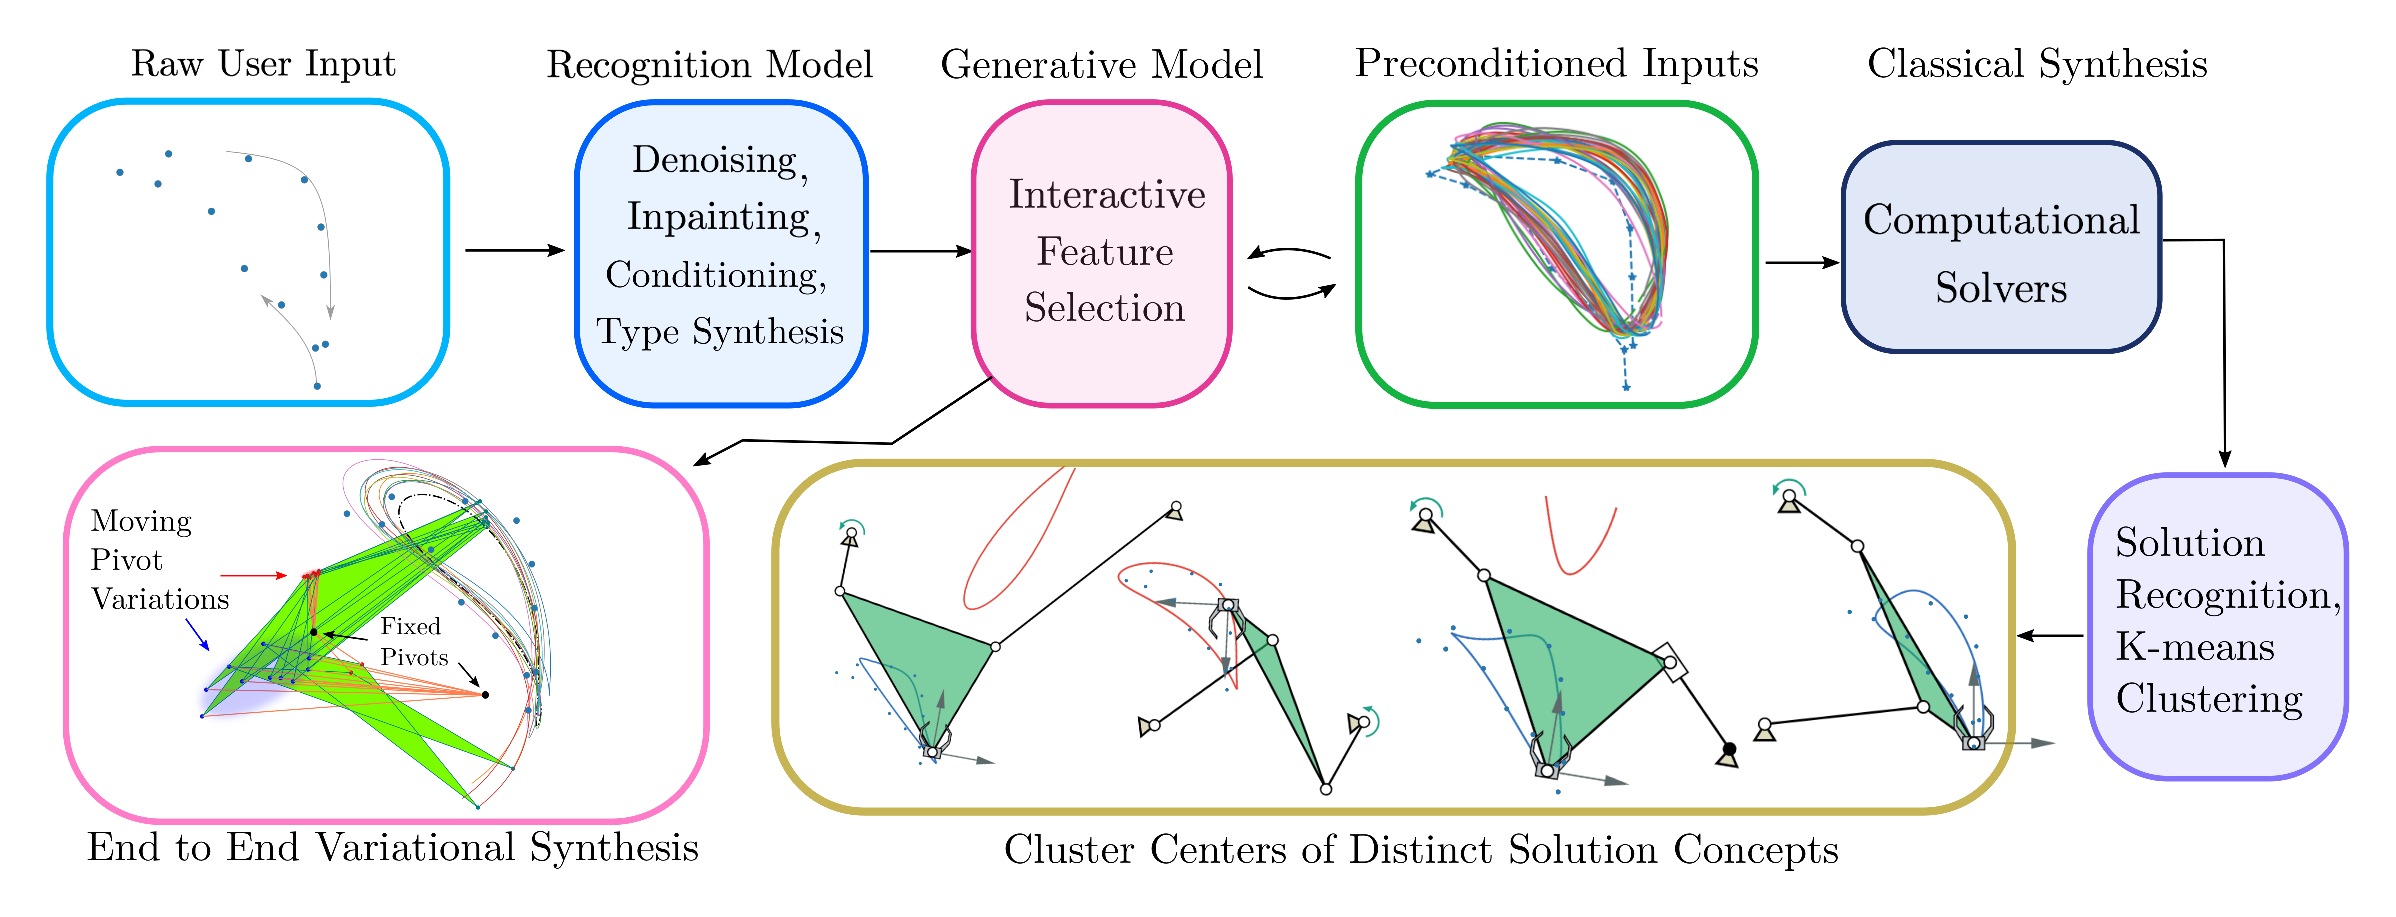
\includegraphics[width=\textwidth]{jmd-19/figure/fig_overview.eps}
  \caption{Crude Input from the user is passed through Recognition Model which captures the features based on which various further actions are determined. The user has the control to override the feature selection by inspecting reformed variational inputs. These variational inputs are passed to classical synthesis methods like ~\cite{generalfitting-JCISE},\cite{shrinathpurwar2017} to generate a multitude of solutions. Solutions are passed through another Recognition and Clustering Module to present the user with distinct distributions of solution concepts. In addition, an End-to-End deep generative model is trained that conditions coupler paths to linkage parameter distributions.}
\label{fig_example_overview}
\end{figure}

\begin{figure*}[tbh]
\centering
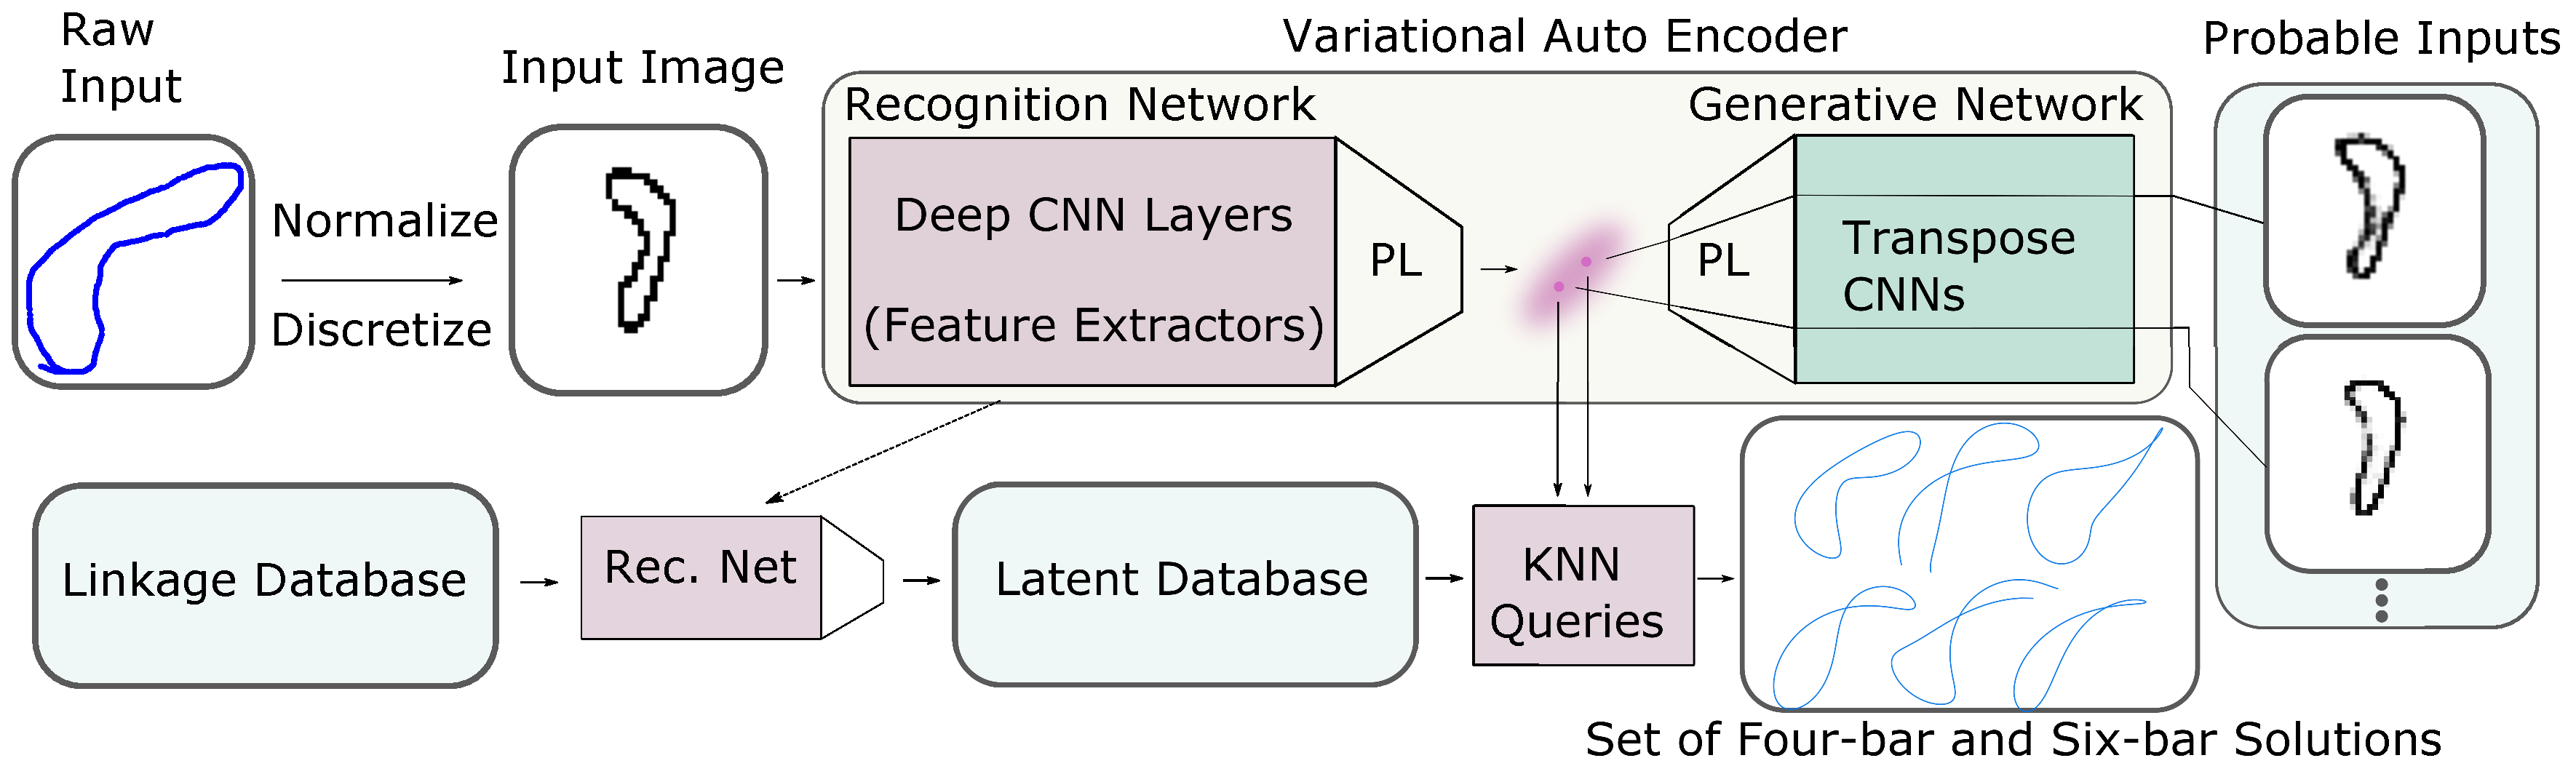
\includegraphics[width=\textwidth]{idetc-20/figure/fig_overview.eps}
  \caption{Overview: Raw input is normalized and discretized into an image. This image is passed through the recognition network of a trained VAE which computes a probability distribution of latent features describing conducive variations of the raw input. Samples from this distribution are queried to find nearest neighbors in a dataset of four-bar and six-bar linkages. The linkages corresponding to the nearest neighbors have coupler curves similar to the conducive variations.}
\label{fig_contrasting_overview}
\end{figure*}

In addition to the general framework, this work also presents a novel image-based approach for path generation, which is particularly amenable to mechanism synthesis when the input from mechanism designers is deliberately imprecise or inherently uncertain due to the nature of the problem. It models the input curve as a probability distribution of image pixels and employs a probabilistic generative model to capture the inherent uncertainty in the input. In addition, it gives feedback on the input quality and provides corrections for a more conducive input. The image representation allows for capturing local spatial correlations, which plays an important role in finding a variety of solutions with similar semantics as the input curve. Figure~\ref{fig_contrasting_overview} shows an overview of this approach.
 


\section{Juxtaposition with Prior Art}

In the case of the Path Generation problem, Ullah and Kota \cite{ullah1997} and Wu et al.\cite{wu2011} have tried to incorporate the prior on user input by means of finding lower harmonic Fourier Descriptors of the path followed by computing link dimensions using optimization methods.
Li et al.\cite{li2016} have developed a Fourier descriptor-based approach for approximate motion generation, which uses the same prior on coupler path.
These methods are relatively robust to spatial variations in input but susceptible to variations in timing information provided by the user.
Sharma and Purwar~\cite{sharma2019optimal} have addressed this issue to some extent by providing a scheme to compute optimal timing for the input points.
However, the above methods are only defined for the synthesis of four-bar linkages with revolute joints.
In contrast to this, our approach is general enough to condition any type of user input and scales to higher-order linkage mechanisms and spatial robots. A key difference in the previous approaches and our approach is that the conditioning on the input is performed by learning the joint probability distribution of input parameters from a database of linkages instead of relying on the fact that four-bar linkages produce curves which have specific harmonic content.

In order to learn such joint probability distributions, we employ a recently developed deep generative model called Variational Auto Encoder (\ac{vae}). It comprises of two neural networks: 1) Recognition Model (also called Encoder) and 2) Generative Model (also called Decoder).
A trained VAE applies the learned prior probability distribution on observed input, thus acting as a posterior inference model. Additional benefits of using VAE are that the learned posterior inference model can also be used for a host of tasks such as denoising, representation, and imputation.

The proposed framework consists of two classes of VAEs.
The first class is trained only on the coupler trajectories, which emphasizes representation learning of coupler paths (or, motions) for conditioning the task.
The second class is trained to learn the joint distributions of mechanisms in order to recognize their salient features, which is used for concept identification and clustering.
A variant of VAE called conditional \ac{cvae} is also developed which can be used to perform End-to-End variational synthesis with deep learning models.

Applications of powerful function approximators like neural networks are not new to the domain of mechanism synthesis. Vasiliu and Yannou \cite{vasiliu2001} have used Artificial Neural Network (ANN) to interpolate the map between the path and link lengths for Grashof four-bar linkages with revolute joints.
Here, ANNs are mainly utilized to memorize the mapping as a means to replace an atlas.
Khan et al.\cite{khan2015} presented an approach where an ANN is used for mapping between Fourier coefficients corresponding to a coupler path and corresponding linkage parameters.
Galan et al.\cite{galan2009} have used a similar approach but instead of using Fourier Coefficients, they have used wavelet descriptors to represent the shape of the path.
All of the above methods use ANNs just as a mapping tool from a closed coupler path to mechanism link ratios.
In contrast to the black box mapping approach of the above methods, we facilitate user interaction with the network by means of interactive manipulation of latent space.
The approach taken by our methods is unsupervised and semi-supervised learning, with an emphasis on representation learning and understanding the probability distribution of coupler trajectories.

Although our approach can work with any number and type of linkages, we have implemented the methods for following topologies 1) four-bar with all revolute joints (RRRR), 2) slider-crank linkage (RR-PR) and its inversion (RR-RP) and 3) Stephenson I and IIIa six-bar with revolute and prismatic joints 4) Janson's Eight bar. 

The organization of the dissertation is as follows. 
Chapter~\ref{ExtendedBurmester} presents the algorithmic developments that incorporate some of the practical constraints in a previously developed task driven simultaneous type and dimensional synthesis framework~\cite{ge2012novel},~\cite{sixbarJMR}. chapter~\ref{ch-ml-2018} presents a novel contribution to database-driven methods for defect-free path and motion synthesis of planar linkages. Chapter~\ref{ch-generative-models} presents the theory behind the choice of using generative models. Chapter~\ref{ch-task-conditioning} presents the application of VAE in task conditioning, which is one of the key contributions of the dissertation. Chapter~\ref{ch-cave-linkage} presents the end-to-end machine learning based synthesis solver that learns a conditional distribution of linkages with respect to the task.  